% TODO: cite https://github.com/niklas-heer/speed-comparison
\documentclass{beamer}
\usepackage{textcomp}
\usepackage[normalem]{ulem}
\usepackage{listings}
\usepackage{dirtytalk}

\title{Warum ist Python so cool\textinterrobang}
\author{Lars Quentin}
\date{26.04.2022}
\usetheme[numbering=none]{metropolis}

\begin{document}
\frame{\titlepage}

% TODO: cite
\section{Wie beliebt ist Python?}
{
  \usebackgroundtemplate{
  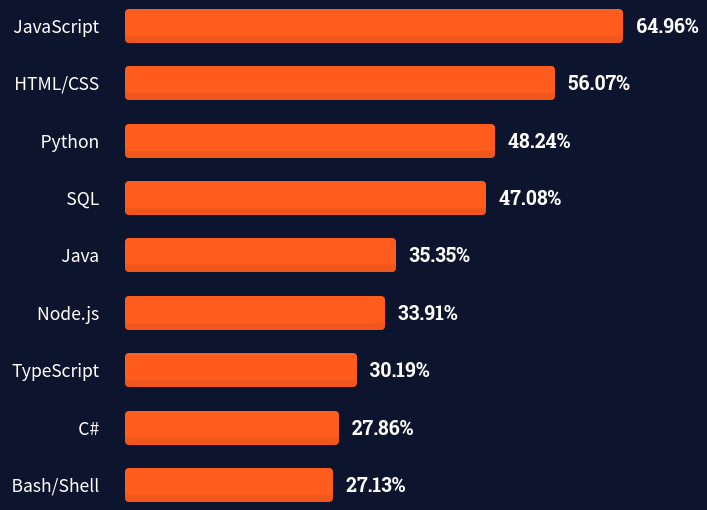
\includegraphics[height=\paperheight,width=\paperwidth]{assets/so1.png}
  }
  \begin{frame}[plain]
  \end{frame}
}
{
  \usebackgroundtemplate{
  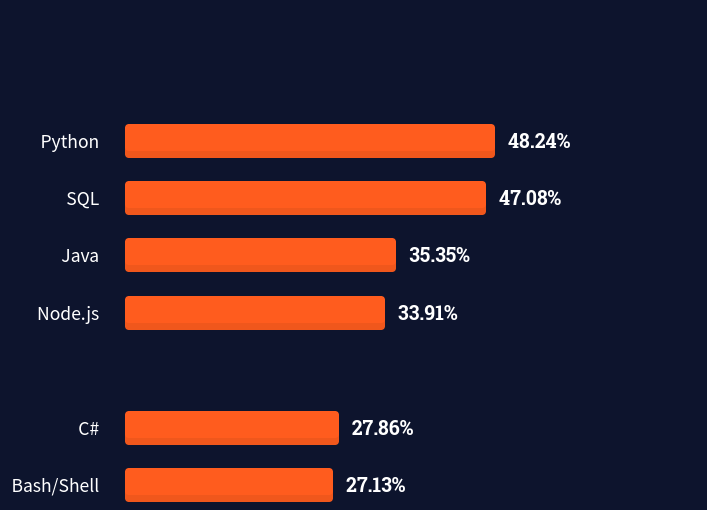
\includegraphics[height=\paperheight,width=\paperwidth]{assets/so2.png}
  }
  \begin{frame}[plain]
  \end{frame}
}
{
  \usebackgroundtemplate{
  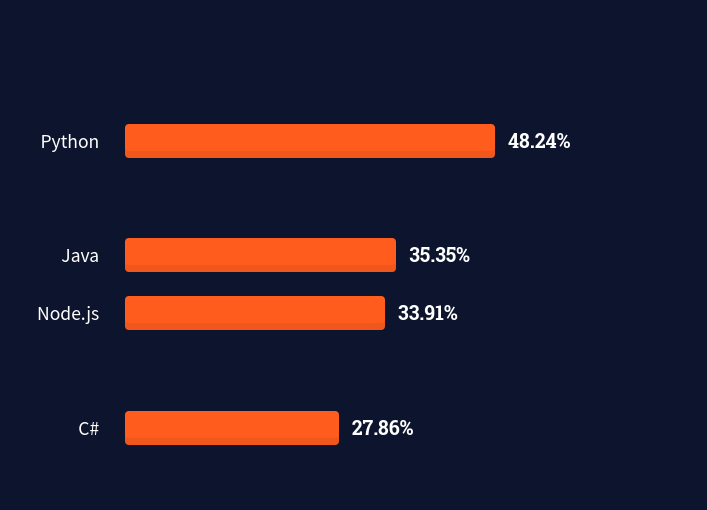
\includegraphics[height=\paperheight,width=\paperwidth]{assets/so3.png}
  }
  \begin{frame}[plain]
  \end{frame}
}

% Warum ich das mache: Dieser Vortrag soll ueber Programmiersprachen gehen.
% Insbesondere soll man hier besondere Konzepte der Sprache vorstellen
\section{Was macht Python so besonders?}
% Erforschen wir mal die Möglichkeiten

\begin{frame}
\begin{center}
{\usebeamerfont*{frametitle} \Huge Plattformexklusivität?}\\~\\
\pause
Nein!
\end{center}
\end{frame}

\begin{frame}
\begin{center}
{\usebeamerfont*{frametitle} \Huge Performance?}
\end{center}
\end{frame}

{
  \usebackgroundtemplate{
  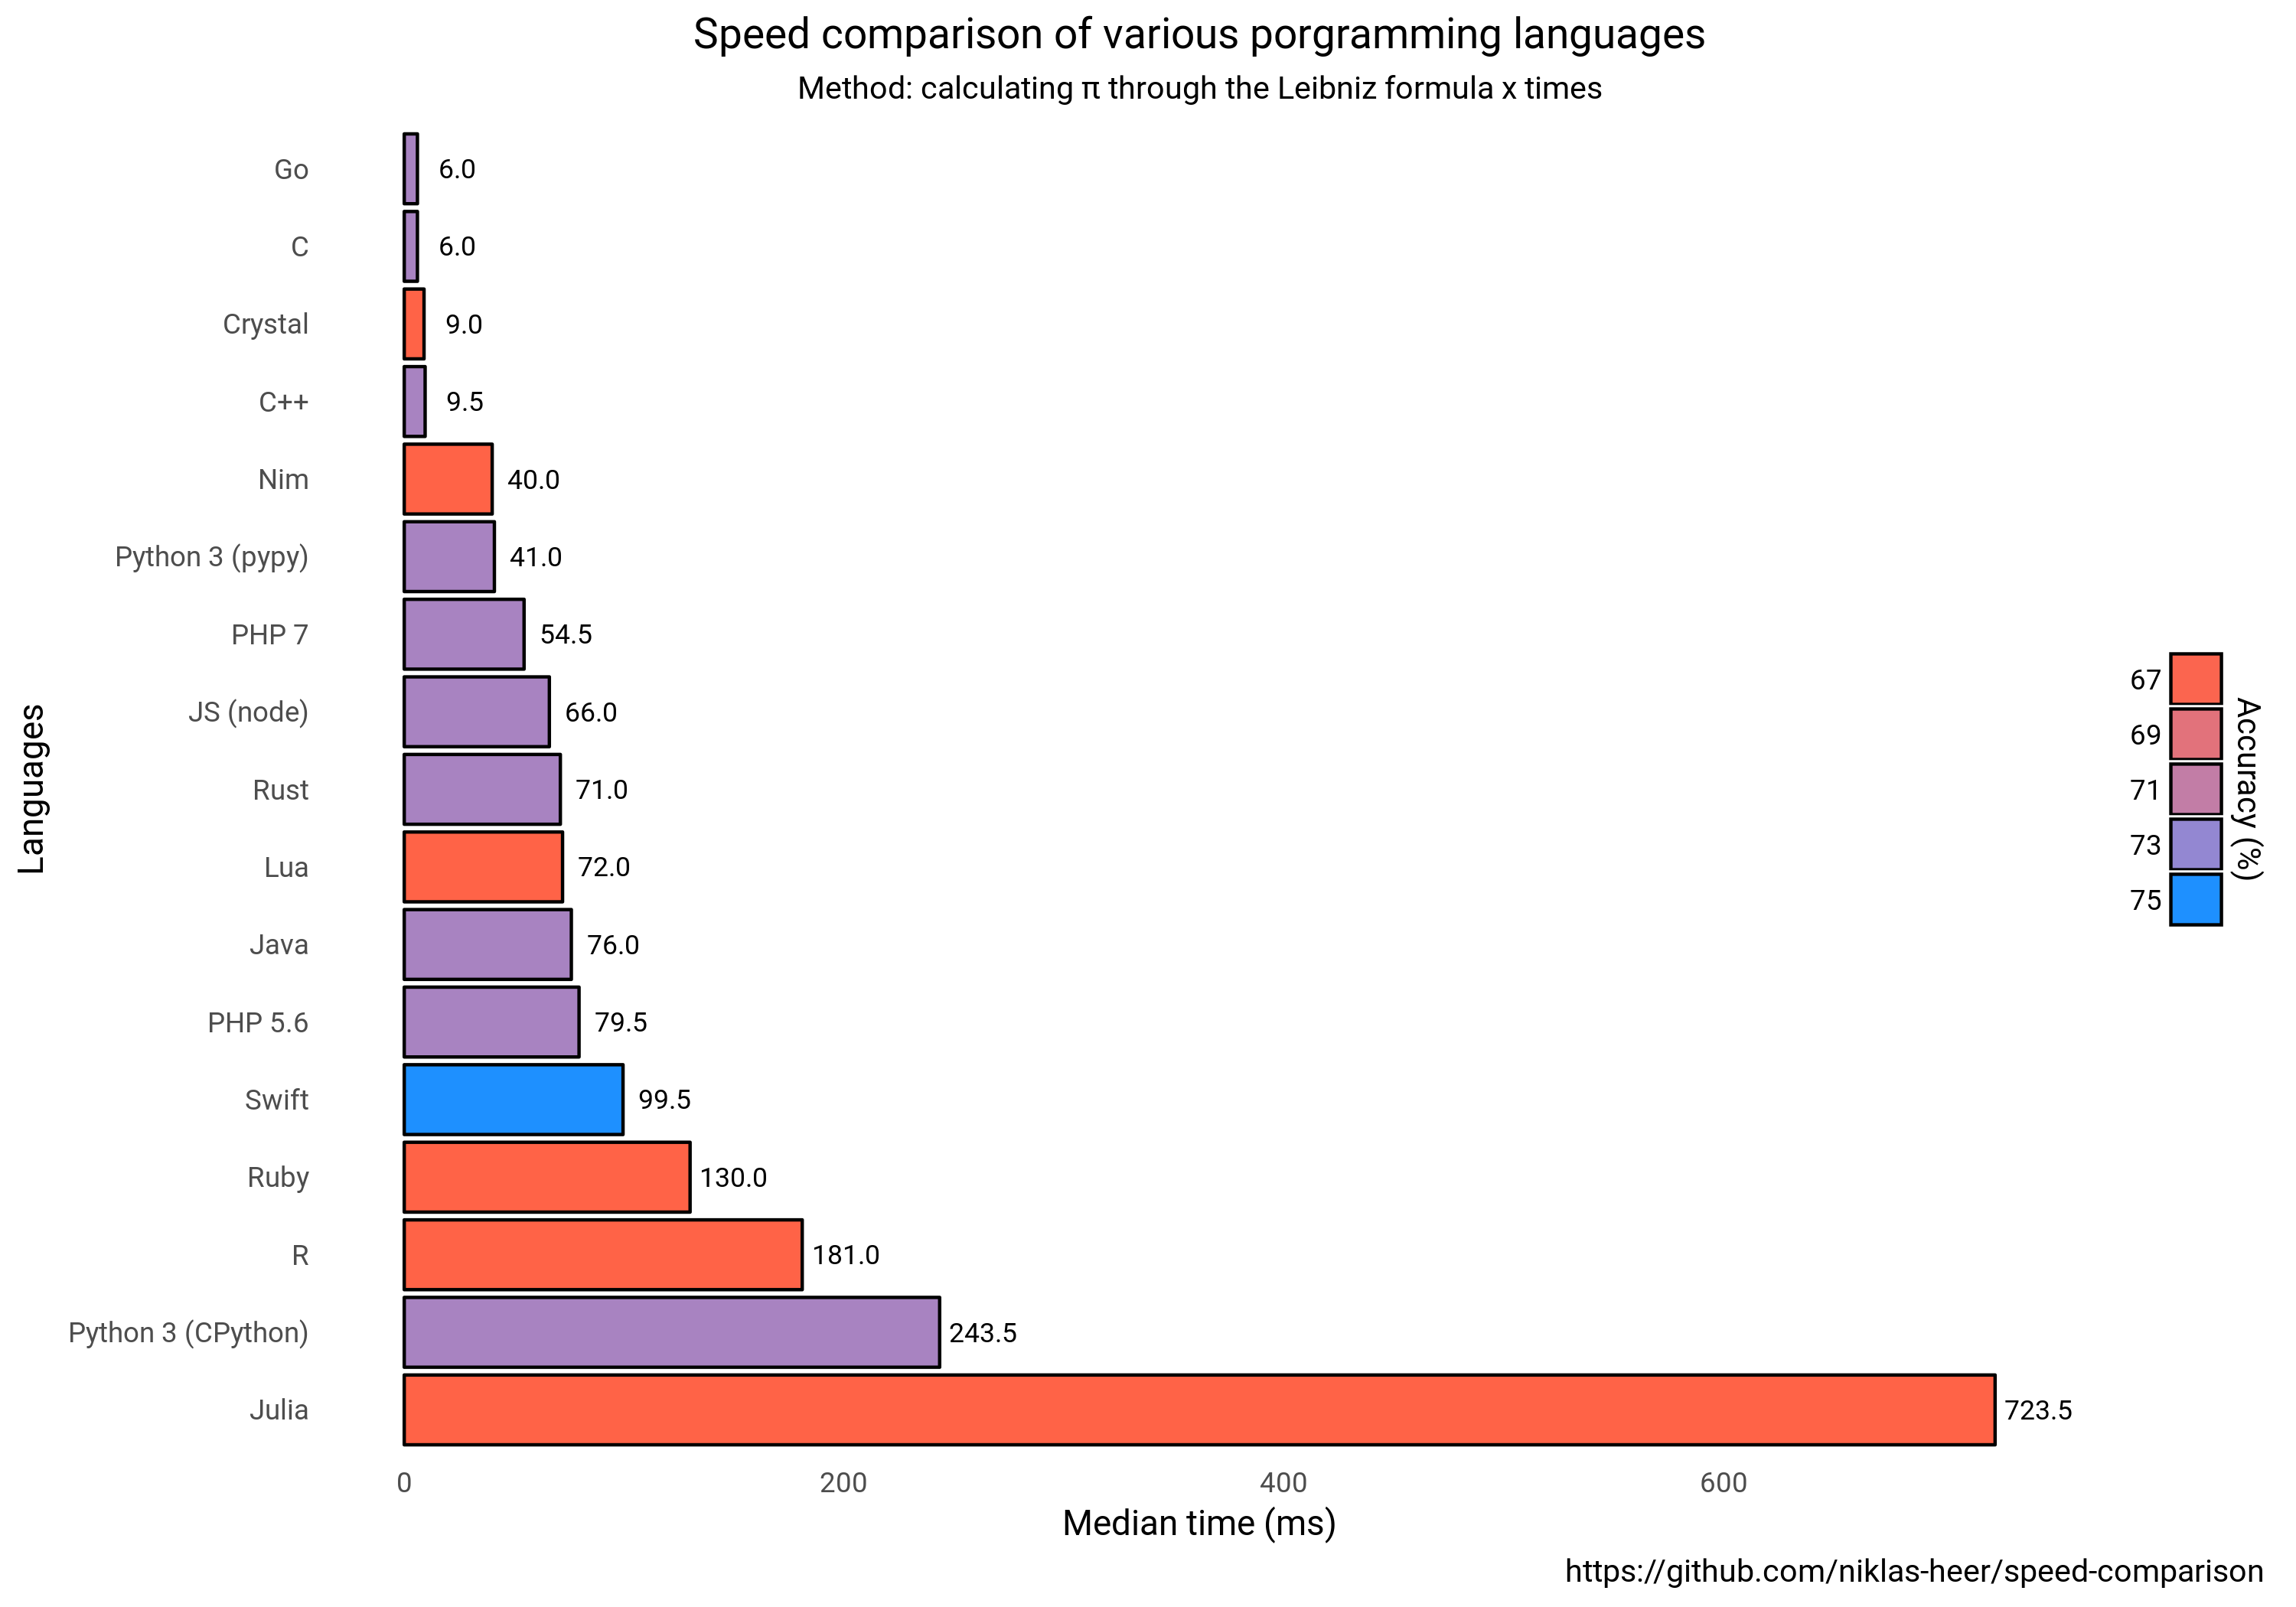
\includegraphics[height=\paperheight,width=\paperwidth]{assets/bench.png}
  }
  \begin{frame}[plain]
  \end{frame}
}

\begin{frame}
\begin{center}
{\usebeamerfont*{frametitle} \Huge Performance?}\\~\\
lol
\end{center}
\end{frame}

\begin{frame}
\begin{center}
{\usebeamerfont*{frametitle} \Huge Libraries?}
\end{center}
\end{frame}

\begin{frame}[t]{Was macht Python so besonders?}
Also... was ist es nun?
\pause
\begin{itemize}
\item \sout{Plattformexklusivität}
\pause
\item \sout{Performance}
\pause
\item Revolutionäre Paradigmen?
\end{itemize}
\end{frame}

\begin{frame}[t]{Was macht Python so besonders?}
Also... was ist es nun?
\begin{itemize}
\item \sout{Plattformexklusivität}
\item \sout{Performance}
\item \sout{Revolutionäre Paradigmen?}
\item Einfach bugfreie Programme zu schreiben? % ne das ist haskell :^)
\end{itemize}
\end{frame}

\begin{frame}[t]{Was macht Python so besonders?}
Also... was ist es nun?
\begin{itemize}
\item \sout{Plattformexklusivität}
\item \sout{Performance}
\item \sout{Revolutionäre Paradigmen?}
\item \sout{Einfach bugfreie Programme zu schreiben?}
\item Besondere Sprachfeatures für ML, Webdev, Web3, Embedded...
\end{itemize}
\end{frame}

% TODO: Einbauen warum "alle libs" kein gutes Argument ist
% Henne-Ei
\begin{frame}[t]{Was macht Python so besonders?}
Also... was ist es nun?
\begin{itemize}
\item \sout{Plattformexklusivität}
\item \sout{Performance}
\item \sout{Revolutionäre Paradigmen?}
\item \sout{Einfach bugfreie Programme zu schreiben?}
\item \sout{Besondere Sprachfeatures für ML, Webdev, Web3, Embedded...}
\end{itemize}
\begin{center}
{~\\~\\\Huge ???????}
\end{center}
\end{frame}

\begin{frame}
\begin{center}
{\usebeamerfont*{frametitle} \Huge Python ist langweilig.}\\~\\
\pause
{\Large Und langweilig ist simpel.}
\end{center}
\end{frame}

\begin{frame}[t]{Aufgabenstellung}
\textbf{Gegeben:}\\
\vspace{0.2cm}
Eine Textdatei mit kommaseparierten Ganzzahlen\\~\\~\\~\\
\textbf{Aufgabe:}
\begin{itemize}
\item Lies die Datei ein
\item Berechne die Summe
\item Berechne die Anzahl der Elemente
\item Gebe den Mittelwert aus
\end{itemize}
\end{frame}

\begin{frame}
\begin{center}
{\usebeamerfont*{frametitle} \Huge Wieso ist Python so gut?}\\~\\
\pause
Vieles!
\end{center}
\end{frame}

\section{Zug\"anglichkeit f\"ur Nicht-Programmierende}

\begin{frame}{Jupyter Notebooks}
\begin{columns}[onlytextwidth,T]
\column{\dimexpr\linewidth-30mm-5mm}
\begin{itemize}
\item Webbasierte Pythonumgebung
\item Interaktiv
\item Grafisch
\item Kostenloses online benutzbar
\begin{itemize}
\item Google Colab
\item Jupyter GWDG
\end{itemize}
\item Open Source, BSD-3 lizensiert
\item Sp\"ater mehr
\end{itemize}
\column{30mm}

\includegraphics[width=30mm]{./assets/jupyter.png}
\end{columns}
\end{frame}

\begin{frame}{Ben\"otigtes Vorwissen}
\begin{center}
\LARGE Was braucht man f\"ur Vorwissen?
\end{center}
\pause
\begin{itemize}
\item Typensysteme? Integergr\"o\ss{}en?
\pause
\item Kommandozeile?
\pause
\item Compiler?
\pause
\item Speicher?
\pause
\item Build Systems?
\pause
\item reinterpret\_cast\textless bool(\_\_stdcall*)(const char*, const char*)\textgreater?
\pause
\end{itemize}
\begin{center}
\Large Englischkenntnisse reichen zum lesen.\\
Einfach Notebook auf und tippen.
\end{center}
\end{frame}

\section{Zug\"anglichkeit f\"ur Programmierende}

% C-Beispiel
\begin{frame}
\begin{center}
\Huge Paradigmenagnostisch
\end{center}
\end{frame}

\begin{frame}
\begin{center}
\Huge Riesige Standard Library
\end{center}
\end{frame}

\begin{frame}{Standard Library}
Was hat die Standard Library alles?
\pause
\begin{itemize}
\item Parser: JSON, CSV, XML
\pause
\item Protokolle: HTTP, FTP, POP3, IMAP4, SMTP
\pause
\item Grafische Interfaces: tkinter
\pause
\item Regul\"are Ausdr\"ucke
\pause
\item SQL(ite)-Interop
\pause
\item Logging Library
\pause
\end{itemize}
POSIX-Tools, SSL-Wrapper, CURSES, GZIP/BZIP2/TAR compression...
\end{frame}

% Viel Variation durch Informatikferne
% Die Standardlibrary gibt den Coding stil vor
% Beispiel: JSON
\begin{frame}
\begin{center}
{\usebeamerfont*{frametitle} \Huge Die Entwickler werden erwachsen}\\
...und entwerfen nun ihre eigenen Libraries.
\end{center}
\end{frame}

\section{Compound Interest}

\begin{frame}{Compound Interest}
\begin{center}
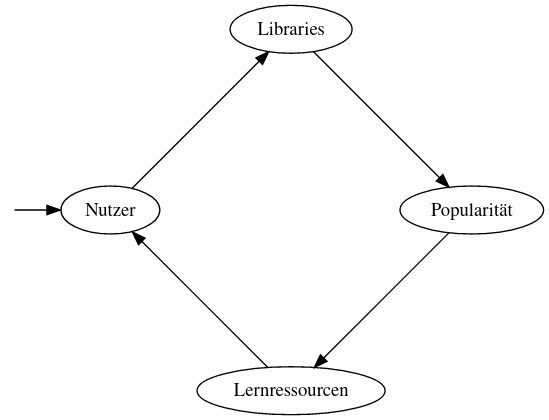
\includegraphics[width=100mm]{assets/circle.png}
\textbf{Endresultat}: Es gibt Libraries/Bindings f\"ur alles.
\end{center}
\end{frame}

\begin{frame}{Compound Interest}
\begin{center}
{\usebeamerfont*{frametitle} \large \say{das Reichtum an Paketen und libs lässt über mögliche Nachteile der Sprache hinwegsehen, weil 50\% der use cases eh nur import + 3 Zeilen eigener Code sind}}\\
\end{center}
-- David Eipper, 2022
\end{frame}

\section{Bonus: Wichtige Bibliotheken}

% TODO Pauses
\begin{frame}{Kategorien}
\Huge
\begin{center}
\begin{itemize}
\item Skripting / Administration
\item GUI-Programmierung
\item Data Science
\item Web-Development
\end{itemize}
\end{center}
\end{frame}

% TODO Pause
\begin{frame}
\begin{center}
\begin{columns}[onlytextwidth,T]
\column{\dimexpr\linewidth-65mm-5mm}
\begin{block}{Scripting}
\begin{itemize}
\item Subprocess
\item Shlex
\item OS
\end{itemize}
\end{block}
\pause
\begin{block}{GUI-Programmierung}
\begin{itemize}
\item tkinter
\item \textbf{PyQT5}
\item pyimgui
\end{itemize}
\end{block}
\pause
\column{65mm}
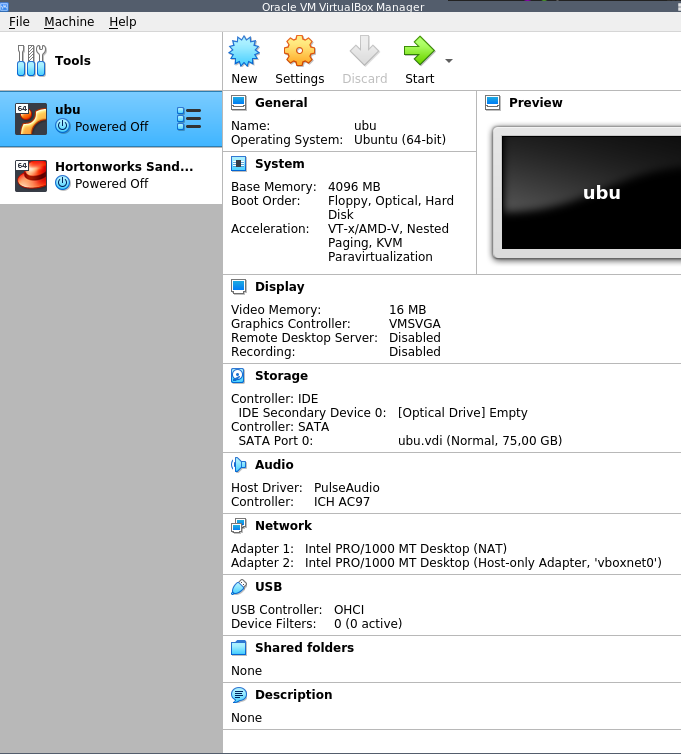
\includegraphics[width=65mm]{./assets/vb.png}
\end{columns}
\end{center}
\end{frame}

\begin{frame}
\begin{center}
\begin{columns}[onlytextwidth,T]
\column{\dimexpr\linewidth-65mm-5mm}
\begin{block}{Data Science}
\begin{itemize}
\pause
\item \textbf{Anaconda}
\pause
\item \textbf{numpy + scipy}
\pause
\item \textbf{matplotlib}
\pause
\item \textbf{pandas}
\pause
\item dask
\pause
\item scikit-learn
\pause
\item keras
\pause
\item BeautifulSoup
\end{itemize}
\end{block}
\column{65mm}
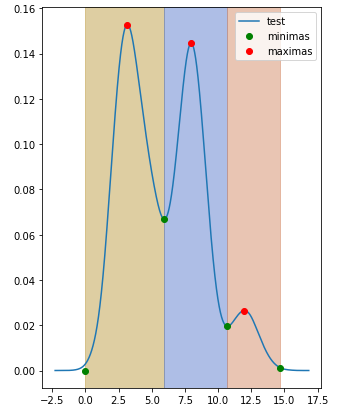
\includegraphics[width=65mm]{./assets/pyplot.png}
\end{columns}
\end{center}
\end{frame}

\begin{frame}
\begin{center}
\begin{block}{Web Development}
\begin{itemize}
\pause
\item \textbf{Flask}
\pause
\begin{itemize}
\item Pinterest
\end{itemize}
\pause
\item \textbf{Django}
\pause
\begin{itemize}
\item Youtube
\item Instagram
\item Dropbox, Spotify, Mozilla, NASA...
\end{itemize}
\pause
\item \textbf{FastAPI}
\pause
\begin{itemize}
\item Microsoft
\item Netflix
\item Uber
\end{itemize}
\pause
\item \textbf{Pelican}
\pause
\item Django-REST
\item Bottle.py
\end{itemize}
\end{block}
\end{center}
\end{frame}

\begin{frame}
\begin{center}
{\usebeamerfont*{frametitle} \Huge Danke f\"ur eure Aufmerksamkeit!}\\
Gleich gehts weiter mit Teil 2 über den Code.
\end{center}
\end{frame}

\end{document}
